%% ****** Start of file apstemplate.tex ****** %
%%
%%
%%   This file is part of the APS files in the REVTeX 4 distribution.
%%   Version 4.1r of REVTeX, August 2010
%%
%%
%%   Copyright (c) 2001, 2009, 2010 The American Physical Society.
%%
%%   See the REVTeX 4 README file for restrictions and more information.
%%
%
% This is a template for producing manuscripts for use with REVTEX 4.0
% Copy this file to another name and then work on that file.
% That way, you always have this original template file to use.
%
% Group addresses by affiliation; use superscriptaddress for long
% author lists, or if there are many overlapping affiliations.
% For Phys. Rev. appearance, change preprint to twocolumn.
% Choose pra, prb, prc, prd, pre, prl, prstab, prstper, or rmp for journal
%  Add 'draft' option to mark overfull boxes with black boxes
%  Add 'showpacs' option to make PACS codes appear
%  Add 'showkeys' option to make keywords appear
\documentclass[aps,prl,groupedaddress,twocolumn]{revtex4-1}
%\documentclass[aps,prl,preprint,superscriptaddress]{revtex4-1}
%\documentclass[aps,prl,reprint,groupedaddress]{revtex4-1}

\usepackage{graphicx}
\usepackage{epsfig}

% You should use BibTeX and apsrev.bst for references
% Choosing a journal automatically selects the correct APS
% BibTeX style file (bst file), so only uncomment the line
% below if necessary.
\begin{document}

% Use the \preprint command to place your local institutional report
% number in the upper righthand corner of the title page in preprint mode.
% Multiple \preprint commands are allowed.
% Use the 'preprintnumbers' class option to override journal defaults
% to display numbers if necessary
%\preprint{}

%Title of paper
\title{Title of Paper}

% repeat the \author .. \affiliation  etc. as needed
% \email, \thanks, \homepage, \altaffiliation all apply to the current
% author. Explanatory text should go in the []'s, actual e-mail
% address or url should go in the {}'s for \email and \homepage.
% Please use the appropriate macro foreach each type of information

% \affiliation command applies to all authors since the last
% \affiliation command. The \affiliation command should follow the
% other information
% \affiliation can be followed by \email, \homepage, \thanks as well.
\author{Your name}
\email[]{your.e-mail@address}
%\homepage[]{Your web page}
%\thanks{}
%\altaffiliation{}
\affiliation{Lund University}

%Collaboration name if desired (requires use of superscriptaddress
%option in \documentclass). \noaffiliation is required (may also be
%used with the \author command).
%\collaboration can be followed by \email, \homepage, \thanks as well.
%\collaboration{}
%\noaffiliation

\date{\today}

\begin{abstract}
Summarize the first three paragraphs in the introduction and each paragraph in the conclusions with one sentence each. Define the topic. Define the gap in the existing knowledge. Describe how you have filled this gap. Summarize your main conclusions. Why is this important and how can it change the world?
\end{abstract}

% insert suggested PACS numbers in braces on next line
% \pacs{}
% insert suggested keywords - APS authors don't need to do this
%\keywords{}

%\maketitle must follow title, authors, abstract, \pacs, and \keywords
\maketitle

% body of paper here - Use proper section commands
% References should be done using the \cite, \ref, and \label commands
%\section{}
% Put \label in argument of \section for cross-referencing
\section{\label{intro}Introduction}
The first paragraph (5-10 lines) shall define the broad topic of the paper. For instance, if the topic is catalysis, define what catalysis is and why it is important. If the paper concerns a certain kind of catalysis, introduce this as well.

The second paragraph (10-20 lines) defines a lack in the present knowledge. For instance, the active phase for CO oxidation is not well known although it has been studied very much. Discuss what others have done in order to fill this knowledge gap. Explain why this is not enough. (Still do not mention what you have done.) (This paragraph may be split in two.)

The third paragraph (5-10 lines) explains what you have done in order to fill the knowledge gap from the previous paragraph. “In order to fill this knowledge gap, we have…” This is the first time (except for the abstract) you mention what you have done.

The fourth paragraph (5-10 lines) previews the rest of the paper. Discuss what you have found (you can, but do not have to, reveal the main results here) and why this is important for the future. (The third and fourth paragraphs may be combined to one.)

\section{Materials and Methods}
Where and how were the measurements/the study done? For instance, "The XPS experiments were done at beamline i311 at the MAX IV laboratory" [reference to paper about the experimental station]? Did you use any special equipment? Were there any special settings, such as photon energy, used throughout the study? Do not mention if it does not apply to all measurements. How were the data analysed? Is there anything special, such as choice of coordinate system, that the reader needs to know about in order to interpret the data in the paper?

What kind of samples were used and how were they prepared?

How were the measurements performed? Again, only discuss common features between all the reported measurements. "In order to investigate the deactivation of the catalyst, the activity was first started by heating the sample in the reaction gas mixture, after which the temperature was lowered slowly until deactivation." Since the gas mixtures were different in the different measurements, I do not mention them.

Anything else that can be important for the outcome of the experiments, that is not obvious from the choice of method or setup? This section should provide enough information for someone who is familiar with the method to be able to judge the quality of the results.


\section{Results}
For each figure, describe in one sentence the general content of the figure. Then guide the reader through the data of the figure and introduce the different subfigures if there are any. This section is supposed to be objective, that is, you should report what is shown in the figure, but not more interpretation than necessary.

"Figure 1 shows the deactivation of the CO oxidation reaction on the epitaxial bulk oxide on Pd(100) during a slow cooling process. The O$_2$:CO ratio was? Panel a shows the CO$_2$ RGA signal (blue), monitoring the catalytic activity, as well as the sample temperature (red). The constant CO$_2$ signal in the beginning shows that the catalytic reaction is active enough to be mass transfer limited, but after about 1700 s, the activity suddenly drops significantly. The temperature drops slightly at the same time, as expected since reaction is very exothermic. Figure 1b shows...  This shows that the Pd oxide is at least as active as the metallic surface."

\begin{figure}
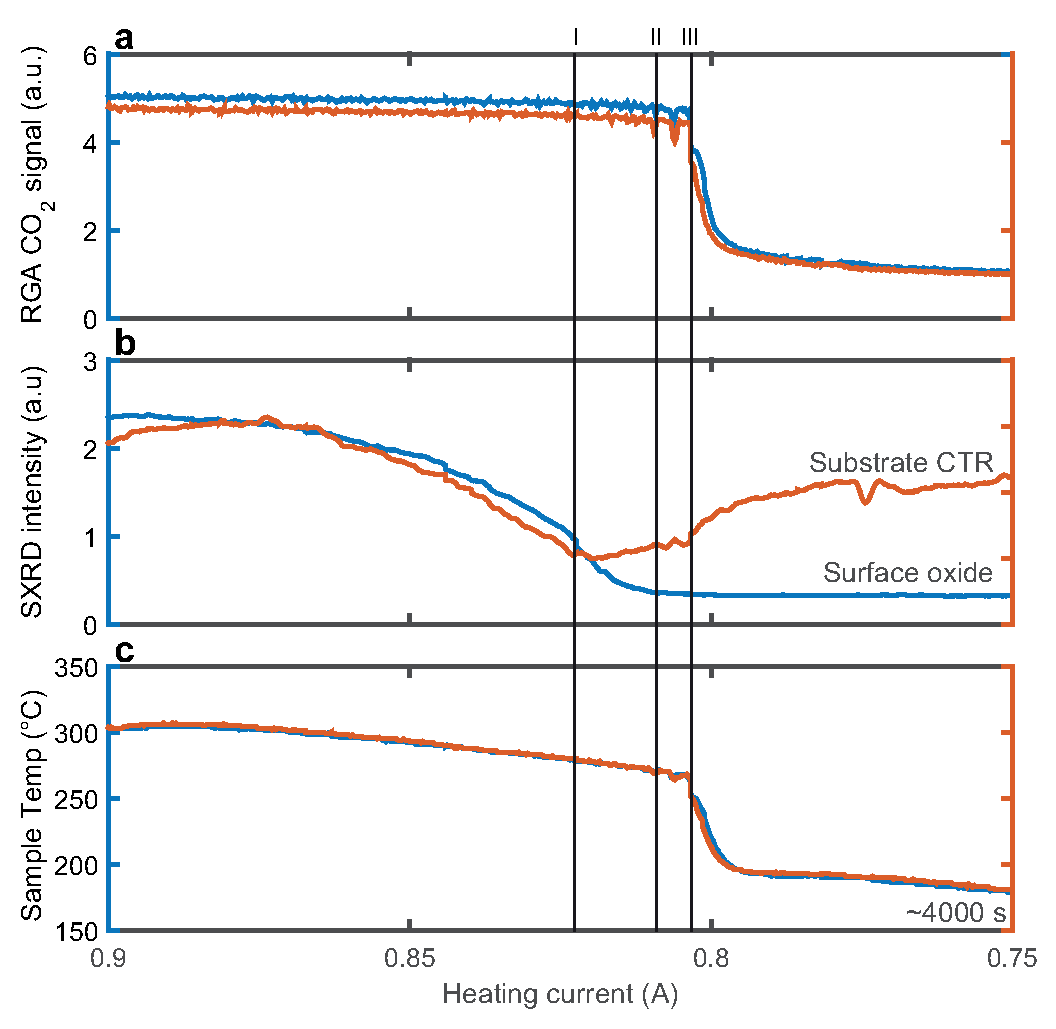
\includegraphics[width=8cm]{rh111-sxrd.eps}
\caption{\label{Fig:1} \textbf{One sentence summarizing the whole figure.} Describe the conditions for the measurements reported in the figure. Describe each of the panels and the data. Preferably, a basic interpretation of the data should be possible from only the figure and the caption. Still it should not be too long, so you have to make your own judgement on how much to include.}
\end{figure}

\section{Discussion}
Summarize the results in one sentence. Discuss for one paragraph how you interpret these data and the main conclusions. Now the discussion does not have to be as objective anymore, and you are allowed to speculate as long as you make this clear.

Mention previous studies of the same or similar systems and how they agree or disagree with the results of this study. It has to be clear from the discussion that your results increase the knowledge in a useful way.

\textit{Our results show that the reaction between CO and preadsorbed O happens at lower temperature on the stepped Rh(553) surface than on flat Rh(111). This is in agreement with the general assumption that the under-coordinated...\cite{Lundgren_2008}}

\section{Conclusions}

Summarize the results and discussion in one sentence. Try to generalize and discuss whether these results, in one way or another, can be valid for other similar, or not so similar, systems.
Discuss how the results can be important. Will your results open up opportunities for further studies? Will they lead to the development of new devices? How will this change the world? Here you are free to speculate quite freely, as long as you are open with it. "This could potentially lead to the end of climate warming?"


\section{Acknowledgments}
I would like to thank...

% Create the reference section using BibTeX:
\bibliography{References}
\bibliographystyle{apsrev4-1}

\end{document}

% \begin{thebibliography}{99}

% \bibitem{lundgren1}
% E. Lundgren, H. Over, \textit{In situ gas-surface interactions: Approaching realistic conditions.} J. Phys.: Condens. Matter \textbf{20} (2008) 180302.

% \end{thebibliography}

% 
%
% ****** End of file apstemplate.tex ******

